% Created 2023-03-24 Fri 00:34
% Intended LaTeX compiler: xelatex
\documentclass[aspectratio=1610,xcolor={dvipsnames},hyperref={colorlinks,unicode,linkcolor=violet,anchorcolor=BlueViolet,citecolor=YellowOrange,filecolor=black,urlcolor=Aquamarine}]{beamer}
\usepackage{graphicx}
\usepackage{grffile}
\usepackage{longtable}
\usepackage{booktabs}
\usepackage{wrapfig}
\usepackage{rotating}
\usepackage[normalem]{ulem}
\usepackage{amsmath}
\usepackage{textcomp}
\usepackage{amssymb}
\usepackage{capt-of}
\usepackage{nicefrac}
\usepackage[dvipsnames]{xcolor}
\usepackage[colorlinks,unicode,linkcolor=violet,anchorcolor=BlueViolet,citecolor=YellowOrange,filecolor=black,urlcolor=Aquamarine]{hyperref}
\usepackage{etoolbox}
\useoutertheme{infolines}
\setbeamertemplate{frametitle}{%
\usebeamerfont{frametitle}\insertframetitle\strut%
\vskip-0\baselineskip%
\leaders\vrule width .95\paperwidth\vskip1pt%
\vskip0pt%
\nointerlineskip%
}

%% T for footer
\setbeamercolor{footlinecolor}{fg=cyan,bg=green}
\setbeamercolor{author in head/foot}{fg=blue}
\setbeamertemplate{footline}{%
\leavevmode%
\hbox{%
\begin{beamercolorbox}[wd=.26\paperwidth,ht=2.25ex,dp=1ex,left]{author in head/foot}%
\hspace*{2ex}\usebeamerfont{author in head/foot} Dept. CSE, UT Arlington
\end{beamercolorbox}%
\begin{beamercolorbox}[wd=.50\paperwidth,ht=2.25ex,dp=1ex,center]{author in head/foot}%
\usebeamerfont{title in head/foot}Scalable Modeling \& Imaging \& Learning Lab (SMILE)
\end{beamercolorbox}%
\begin{beamercolorbox}[wd=.24\paperwidth,ht=2.25ex,dp=1ex,right]{date in head/foot}%
\usebeamerfont{date in head/foot}
\insertshortdate{}\hspace*{1em}  % date
\insertframenumber/\inserttotalframenumber\hspace*{2ex}
\end{beamercolorbox}}%
\vskip0pt%
}
\setbeamerfont{footnote}{size=\tiny}
\usepackage{minted}
\usetheme{default}
\usefonttheme{serif}
\useinnertheme{circles}
\author{Nasy}
\date{Mar 24, 2023}
\title{Tuning}
\hypersetup{
 pdfauthor={Nasy},
 pdftitle={Tuning},
 pdfkeywords={},
 pdfsubject={},
 pdfcreator={Emacs 29.0.50 (Org mode 9.5.5)}, 
 pdflang={English}}
\usepackage{biblatex}
\addbibresource{~/.emacs.d/萚兮/時/refs/ref.bib}
\begin{document}

\maketitle
\begin{frame}{Outline}
\tableofcontents
\end{frame}


\section{Introduction}
\label{sec:org88782c5}

\begin{frame}[label={sec:org073d86e}]{Introduction}
\begin{description}
\item[{Target:}] Maximizing the performance of the model.
\item[{Question?}] How to get good results with deep learning?
\item[{Why?}] My model does not work!!!
\end{description}

\begin{center}
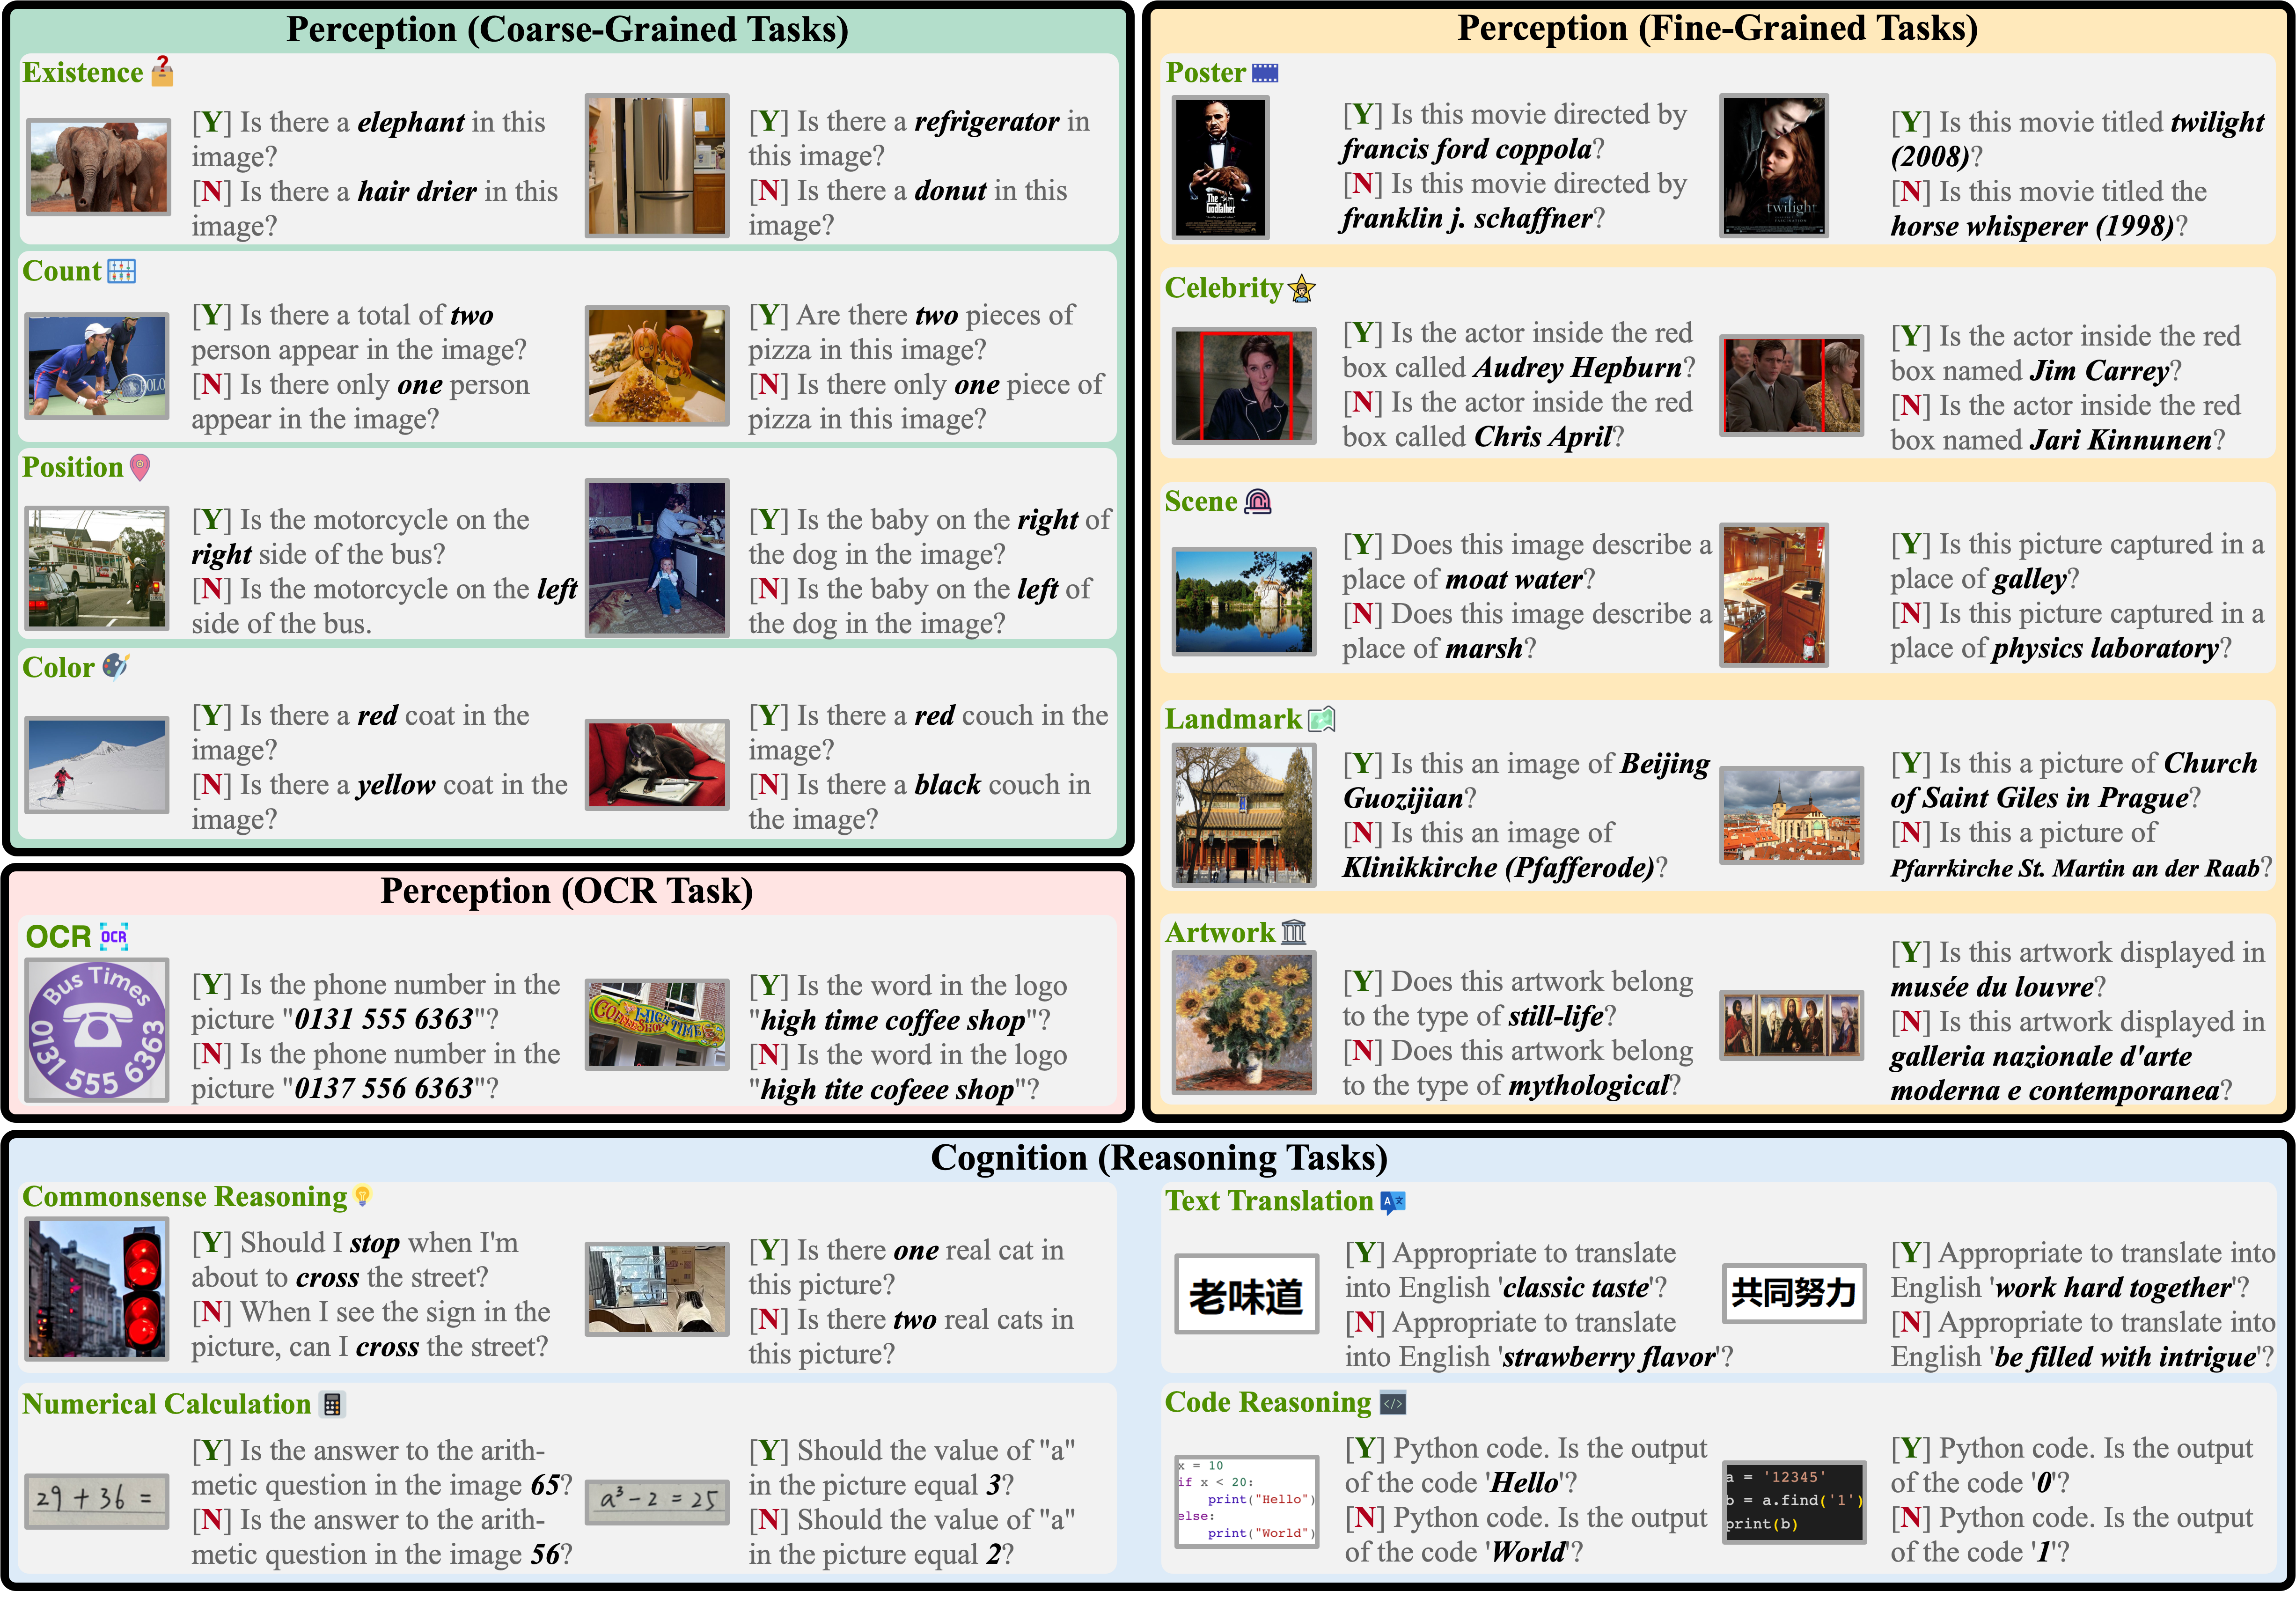
\includegraphics[width=.9\linewidth]{./p1.png}
\end{center}
\end{frame}

\section{Get Start}
\label{sec:orgb4da06c}

\begin{frame}[label={sec:org4b36724}]{Get Start}
\begin{itemize}
\item Model Architecture
\item Optimizer
\item Batch Size
\item Hyperparameters
\begin{itemize}
\item Initial Learning rate, momentum, weight decay, etc.
\end{itemize}
\item ref \footfullcite{DeepLearningTuning2023}
\end{itemize}
\end{frame}

\begin{frame}[label={sec:orgfcae7ae}]{Model Architecture}
\begin{itemize}
\item \large Try to reuse the existing models that already work.

\item Not only the model layers, but also the hyperparameters settings.
\end{itemize}
\end{frame}

\begin{frame}[label={sec:orgb5e8f76}]{Optimizer}
No optimizer is the "best" across all types of machine learning problems and model architectures. \footfullcite{choiEmpiricalComparisonsOptimizers2020}

\begin{center}
\includegraphics[width=.9\linewidth]{./p2.png}
\end{center}
\end{frame}

\begin{frame}[label={sec:org7aa129d}]{Batch Size}
\begin{itemize}
\item Only affects the speed of training.
\item The batch size should not be treated as a tunable hyperparameter. \footfullcite{shallueMeasuringEffectsData2019}
\item In most case, batch size should be the largest batch size supported by the available hardware.
\item Do not change during tuning.
\begin{itemize}
\item Some layers, like the Batchnorm, will be affected.
\end{itemize}
\end{itemize}
\end{frame}

\begin{frame}[label={sec:org06d3840}]{Initial Hyperparameters}
\begin{columns}
\begin{column}{0.4\columnwidth}
Before we start tuning hyperparameters:

\begin{itemize}
\item Model ready (e.g. num of layers).
\item Max traning steps
\item Pipeline ready (e.g. preprocessing, evaluation.)
\end{itemize}
\end{column}

\begin{column}{0.4\columnwidth}
Select the initial hyperparameters:

\begin{itemize}
\item Learning rate (start from fix instead of schedule)
\item Optimizer parameters
\begin{itemize}
\item Adam: lr, beta1, beta2, weight\_decay
\item SGD: lr, momentum, weight\_decay
\end{itemize}
\item Layers parameters
\begin{itemize}
\item Batchnorm: momentum, epsilon
\item Dropout: rate
\item Conv2D: kernel\_size, strides, padding, activation
\item Dense: activation, output features
\item leaky\_relu: alpha
\end{itemize}
\item Search spaces
\end{itemize}
\end{column}
\end{columns}
\end{frame}

\section{Tuning}
\label{sec:org0516a21}

\begin{frame}[label={sec:org50eabc2}]{Hyperparameters}
\begin{description}
\item[{Scientific hyperparameters}] For ablation study. (e.g. num of GCN layers)
\item[{Nuisance hyperparameters}] Optimized for fair comparison for scientific hyperparameters.  (e.g. optimizer parameters)
\item[{Fixed hyperparameters}] No need to change when comparing scientific hyperparameters. (e.g. batch size)
\end{description}
\end{frame}

\begin{frame}[label={sec:orgbca7d5e}]{Strategies}
\begin{itemize}
\item Grid search
\begin{itemize}
\item Small search spaces
\end{itemize}
\item Random search
\begin{itemize}
\item Explore the search space
\end{itemize}
\item Quasi-random search
\begin{itemize}
\item Explore the search space (like the boundary of search space)
\end{itemize}
\item Bayesian optimization
\begin{itemize}
\item Exploit the correlation between hyperparameters.
\item TPE
\item Gaussian process
\item \ldots{}
\end{itemize}
\end{itemize}
\end{frame}

\begin{frame}[label={sec:orgcac1dc7}]{Tuning Tools}
\begin{description}
\item[{Optuna}] \url{https://github.com/optuna/optuna}
\item[{NNI}] \url{https://github.com/microsoft/nni}
\item[{Vizier}] \url{https://github.com/google/vizier}
\item[{hyperopt (outdated)}] \url{https://github.com/hyperopt/hyperopt.git}
\item[{advisor (outdated)}] \url{https://github.com/tobegit3hub/advisor.git}
\end{description}
\end{frame}

\section{Bayesian Optimization}
\label{sec:orge41e0f7}

\begin{frame}[label={sec:org60f90c2}]{Bayesian Optimization}
We have a set of hyperparameters \(X=x_{1}, x_{2},...,x_{n}\), and we want to find the best one for function \(f: x \rightarrow R\), where \(x \in X\):

\[x^* = \arg \max_{x \in X} f(x)\]
\end{frame}

\begin{frame}[label={sec:orgf2a9dac},fragile]{Algorithm}
 \begin{description}
\item[{Input}] \(f\), \(X\), \(S\), \(M\)
\item[{f}] The blackbox function we want to optimize.
\item[{X}] The hyperparameters we want to tune.
\item[{S}] Acquisition function
\item[{M}] Model of BO.  ( Gaussian process; TPE; Random forest; \ldots{} )
\end{description}

\begin{minted}[]{python}
def algorithm(f, X, S, M):
    D = init_samples()  # initial x and y = f(x)
    for i in range(100):
        p = M.fit(D)  # p(y|x, D)
        new_x = S(X, p)
        new_y = f(new_x)
        D.append((new_x, new_y))
\end{minted}
\end{frame}

\begin{frame}[label={sec:org5c06010}]{Acquisition Function}
\begin{itemize}
\item An inexpensive function that can be evaluated at a given point that is commensurate with how desirable evaluating f at x is expected to be for the problem
\item Probability of improvement
\item Expected improvement
\item Entropy search
\item Gaussian Process-Upper Confidence Bound
\end{itemize}
\end{frame}

\section{Refs}
\label{sec:org9a854c5}

\begin{frame}[allowframebreaks]{Refs}
\printbibliography
\end{frame}
\end{document}